\chapter{LAPS}
\section{Einleitung}
Local Administrator Password Solution (LAPS)

\subsection{Anforderungen}
Um LAPS einsetzten zu können, wir ein Active Directory benötigt.

\section{Installation}
Die Installation ist in drei Schritte unterteilt.
Als erstes wird LAPS per Group Policy auf allen Windows Geräten installiert.
Danach wird das Active Directory für LAPS vorbereitet.
Das Active Directory braucht noch zwei zusätzliche Attribute auf den Computer Objekten. 
\begin{itemize}
    \item \textbf{ms-Mcs-AdmPwd}: Speicher das Administrator Passwort in Plain-Text
    \item \textbf{ms-Mcs-AdmPwdExpirationTime}: Speichert den Zeitpunkt für den Passwortwechsel.
\end{itemize}

Zum Schluss wird LAPS per Group Policy aktiviert.

\subsection{Softwareverteilung}

\begin{enumerate}
    \item LAPS kann auf der \href{https://www.microsoft.com/download/details.aspx?id=46899}{Webseite von Microsoft}\footnote{Link: https://www.microsoft.com/download/details.aspx?id=46899} heruntergeladen werden.
    \item Die Datei muss in einem freigegebenen Netzlaufwerk auf dem Domain Controller platziert werden, auf welches alle Computer Zugriff haben.
    Zum Beispiel: \textbf{C:\textbackslash Windows\textbackslash SYSVOL\textbackslash sysvol\textbackslash <domain>\textbackslash}. 
    Dieses Verzeichniss ist Standardmässig freigegeben.
    \item Im Group Policy Management muss eine neue Group Policy erstellt werden, welche mit der OU verknüpft ist, die alle Windows Geräte enthält.
    \begin{figure}[H]
        \centering
        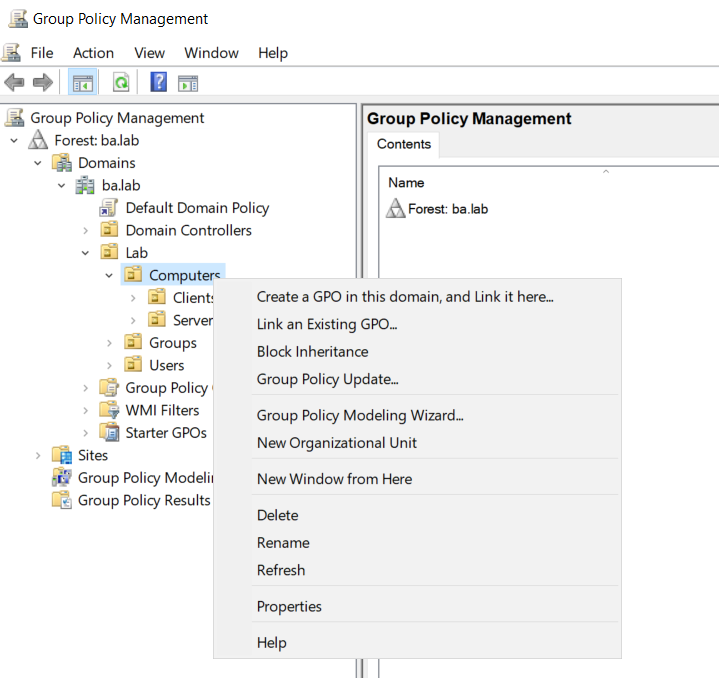
\includegraphics[width=0.7\linewidth]{../img/LAPS/GPO-Create-New.png}
        \caption{Neue GPO für LAPS Deployment}
    \end{figure}
    \item Mit \textbf{Rechtsklick $\rightarrow$ Edit} kann die neue Group Policy bearbeitet werden.
    Unter \textbf{Computer Configuration $\rightarrow$ Policies $\rightarrow$ Software Settings $\rightarrow$ Software installation} kann mit \textbf{Rechtsklick $\rightarrow$ New $\rightarrow$ Package\dots} eine Datei ausgewählt werden, welche installiert werden soll.
    Hier muss man die zuvor im freigegebenen Netzlaufwerk abgelegte Installationsdatei auswählen.
    \begin{figure}[H]
        \centering
        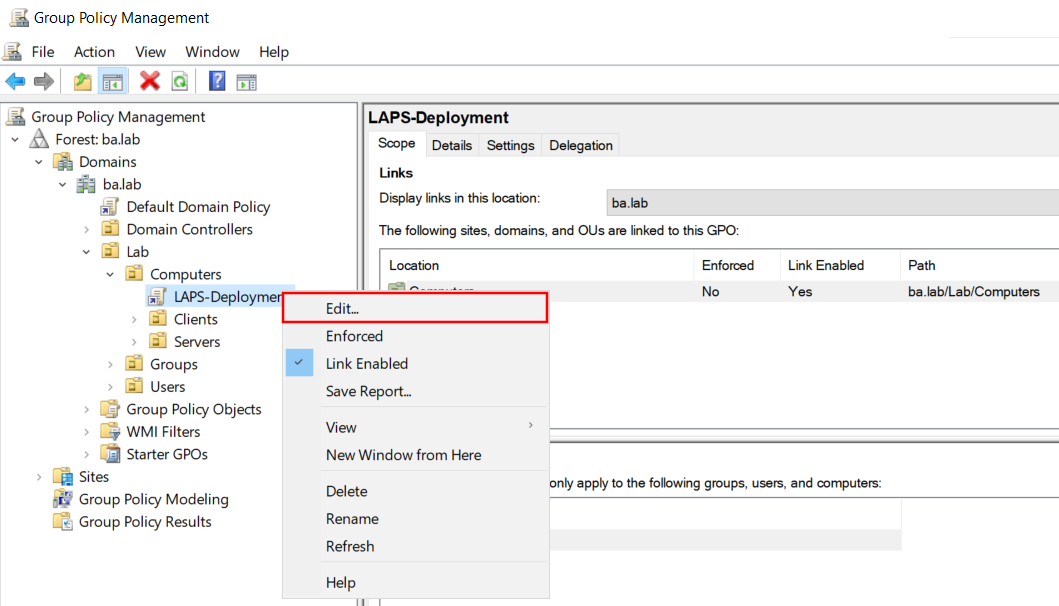
\includegraphics[width=0.7\linewidth]{../img/LAPS/GPO-Edit-Deployment.png}
        \caption{Neue GPO für LAPS Deployment}
    \end{figure}
\item Die Group Policy kann nun geschlossen werden. LAPS wird beim Einloggen auf allen Geräten installiert. Die Installation kann auch mit ``gpupdate /force'' in Powershell/CMD gestartet werden.
\end{enumerate}

\subsection{LAPS GUI für Admins}
Über die GPO wird auf den Computern LAPS ohne GUI installiert.
Mit dem GUI kann man das Passwort von beliebigen Windows Geräten abfragen.

\begin{enumerate}
    \item In der Programmliste in den Systemeinstellungen auf LAPS klicken und im Balken auf \textbf{Change} klicken.
    \begin{figure}[H]
        \centering
        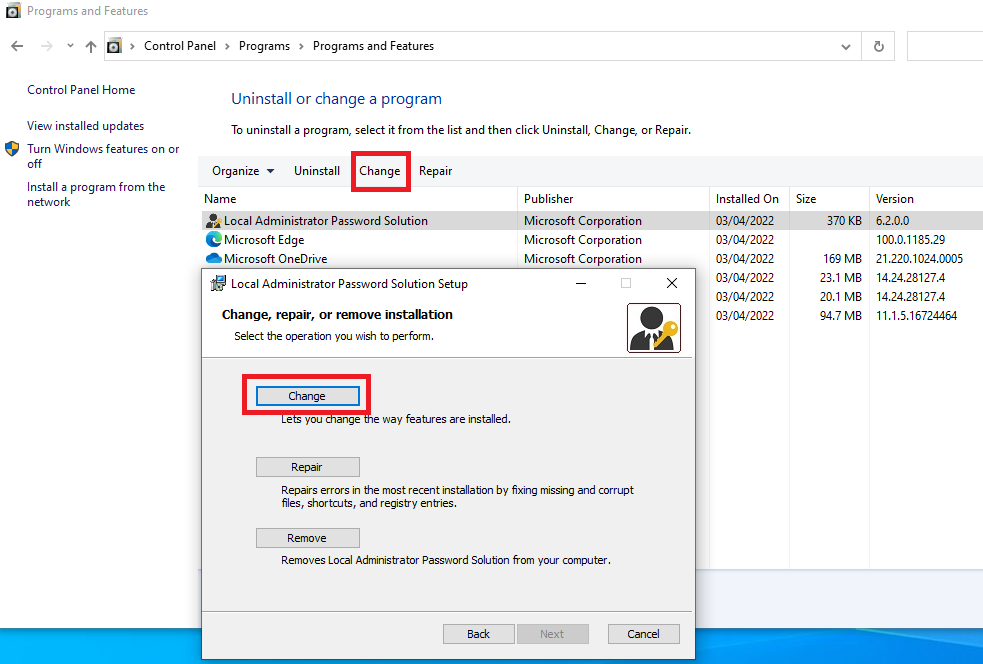
\includegraphics[width=0.7\linewidth]{../img/LAPS/laps-ui-install.png}
        \caption{LAPS GUI Installieren 1}
    \end{figure}

    \item Das \textbf{Management Tools} Feature auswählen und dem Installationsprozess folgen.
    \begin{figure}[H]
        \centering
        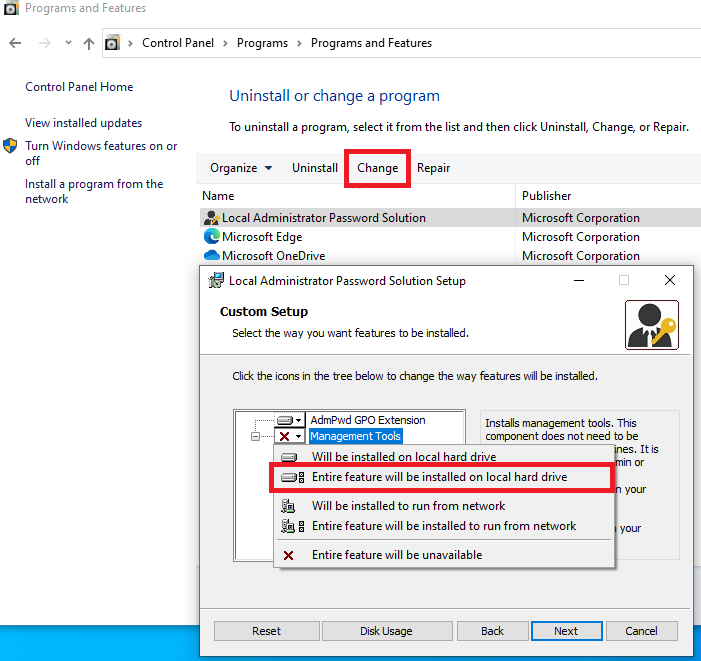
\includegraphics[width=0.7\linewidth]{../img/LAPS/laps-ui-install-2.png}
        \caption{LAPS GUI Installieren 2}
    \end{figure}
\end{enumerate}

\section{Active Directory vorbereiten}
Die zusätzlichen Extension Attributes können per Powershell hinzugefügt werden.
Der Auszuführende Benutzer muss dafür ``Schema Admin'' sein.

\begin{enumerate}
    \item Powershell mit dem Schema Admin Benutzer starten.
    \begin{lstlisting}
Import-module AdmPwd.PS
Update-AdmPwdADSchema

#Resultat:
Operation            DistinguishedName                                              Status
---------            -----------------                                              ------
AddSchemaAttribute   cn=ms-Mcs-AdmPwdExpirationTime,CN=Schema,CN=Configuration,DC=b Success
AddSchemaAttribute   cn=ms-Mcs-AdmPwd,CN=Schema,CN=Configuration,DC=ba,DC=lab       Success
ModifySchemaClass    cn=computer,CN=Schema,CN=Configuration,DC=ba,DC=lab            Success

Set-AdmPwdComputerSelfPermission -OrgUnit "<Name der OU>"
#Resultat:
Name                 DistinguishedName                                              Status
----                 -----------------                                              ------
Clients              OU=Clients,OU=Computers,OU=Lab,DC=ba,DC=lab                    Delegated
    \end{lstlisting}

\end{enumerate}

%3. Create a Group where all Users are added, that can use LAPS. [Laps-Admins.png]
%
%4. Open ASedit [ASEdit.png] and Open Properties of OU with Computers. Open Security tab. Add Group and give ``All Extended Rights''
%Remove All Extended Rights on unneeded accounts
%
%5. Run:
%
%Set-AdmPwdReadPasswordPermission -OrgUnit "Clients" -AllowedPrincipals Global_LAPS-Admins
%Set-AdmPwdResetPasswordPermission -OrgUnit "Clients" -AllowedPrincipals Global_LAPS-Admins

%6. Check Permission:
%
%Find-AdmPwdExtendedrights -identity "Clients"
%
%
%\section{Enforce with GPO}
%
%1. Open GPO Editor on DC and Create a new GPO+Link to all Computer OUs
%
%2. Edit Policy and go to Computer Configuration > Policies > Administrative Templates > Laps [enable-laps]
%
%3. Enable Password Settings and define how: best 14 characters and change all
%
%
%